\documentclass{article}
\usepackage{graphicx}
\begin{document}

\title{ExaSAT: Exascale Static Analysis Tool}

\maketitle
\date

\begin{abstract}
The ExaSAT tool is developed to automatically analyze and compute key performance-related 
metrics for a given code. The tool is composed of two subtools. 
The first tool, developed on top of ROSE compiler framework, performs static compiler analysis and focuses on 
loops and their floating point and memory operations. The collected information from the compiler analysis 
is stored in an XML format. The XML output is fed to the second tool which generates a spreadsheet containing estimated performance 
data and a loop dependency graph. The spreadsheet allows users to enter architecture 
specific parameters such as cache size or memory bandwidth.
The spreadsheet will update the estimated time accordingly.  
We currently implemented the compiler analysis tool for Combustion codes written in Fortran. 
 
\end{abstract}

\section{Static Analysis Description}
With the help of the ExaSAT tool, we would like to answer questions about the performance of 
combustion codes on future architectures. Some of the questions we would like our tool to answer are:
\begin{itemize} 
\item how much data must be moved?
\item how sensitive is the code to memory bandwidth?
\item what is the fraction of communication in overall running time?
\item what is my working set size?
\item etc.
\end{itemize}

\begin{figure}
\begin{center}
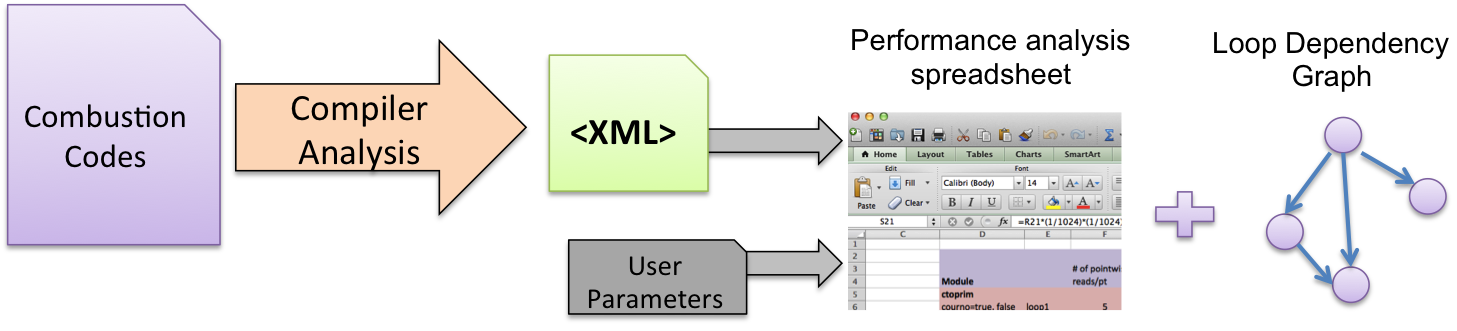
\includegraphics[width=1.0\textwidth]{figs/workflow.png}
\caption{Overview of the ExaSAT tool}
\label{fig:workflow}
\end{center}
\end{figure}

\subsection{Compiler Analysis}
We have developed the compiler analysis using the ROSE compiler framework. 
The compiler analysis tool collects information per function (subroutine or module) and it further 
collects more detail information for nested loops in a function. 
The information collected at the function level includes: 

The information collected at the loop level includes:


\subsection{XML Description}

The results from the first part of the static analysis toolchain
are output in an XML format to interface with the other parts of the
toolchain.  The information in the XML file includes:
\begin{itemize}
\item List
\item of things
\item in the
\item XML
\end{itemize}
Please see the separate XML document detailing the structure of the XML.

\section{Performance Model}

\subsection{Working Sets and Bandwidth Consumption}

{\it Note: in the following analysis, the cache is assumed to have an
ideal LRU eviction policy.  Since real architectures do not have ideal
LRU policies, the analysis of the cache hit rate and resulting memory
traffic is only an approximation of what will be observed in practice.}

Each array may have a different access pattern, so the tool computes
working set and bandwidth usage for each array independently given the
array's access pattern.  The number of planes and pencils in the working
set and bandwidth calculations are different because the number of unique
items that require space in cache to enable reuse may be different from
the number of unique items accessed during a single sweep due to gaps
in the access pattern.

The proper working set size that is both necessary and sufficient to
enable maximum reuse between pencil or plane iterations equals the span
of the pattern plus the maximum gap size across ALL patterns accessed
in the loop.  For example, a stencil pattern that accesses planes -2,
-1, 0, +1, +2, has a working set of 5 planes because there's no gap,
but a pattern of -2, -1, +1, +2 requires a working set of 6 planes for
reuse between plane sweeps even though it only accesses 4 unique planes
during a single sweep.  It may seem counter-intuitive that accessing
fewer planes can increase the working set size, but gaps in the pattern
require the cache to ``remember'' some of the data for a longer period
of time without evicting it.  This requirement can cause an increase in
the working set size.

A similar calculation for pencils is done to enable reuse between
pencil sweeps, but since the pattern for pencils is 2D, we consider each
unique plane in the pattern when computing the maximum gap and working
sets sizes.

\subsection{Dependency Graph Description}

A dependency graph for each function is generated that shows the
dependencies between loops (or solvers) in the function.  Flow,
anti, and output dependencies are considered across all arrays read
and written in each loop.  An example dependency graph is shown in
Figure~\ref{fig:depGraph}.

\begin{figure}
\begin{center}
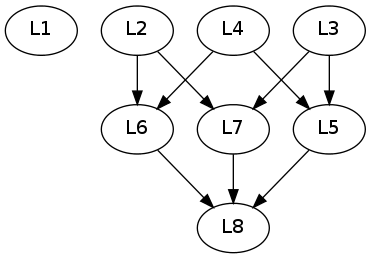
\includegraphics[width=.5\textwidth]{figs/diffterm.png}
\caption{Dependency graph between loops in function {\tt diffterm}
in CNS code {\tt advance.f90.}}
\label{fig:depGraph}
\end{center}
\end{figure}

\subsection{Spreadsheet Description}

\subsubsection{Overview}

At the top of the spreadsheet, there's a table of user-modifiable
parameters.  User-modifiable parameters allow you to change problem
parameters including problem size and cache blocking factor in addition
to machine architecture parameters like Gflop/s/core, GB/s/chip,
and cache/core.  The rest of the spreadsheet updates itself to reflect
the changes made by the user.

The first section beneath the parameters is a loop-level analysis table
listing properties for each loop in the code, including iteration size,
block size, flop counts, working set size, estimated bandwidth usage,
and estimated execution time for each loop.  Totals for the whole program
are also included.

The second section breaks out the analysis for each of the read-only
arrays in each loop because they have ghost cell accesses.  The numbers
computed in this section are then used in the total working set and
bandwidth calculations in the first section.

\subsubsection{Parameters}

The parameters at the top allow the user to explore different settings:

Changing the blocking factor may decrease execution time if it enables
greater reuse of cached data.  On the other hand, increasing the
blocking factor by too great an amount could hurt performance, as there
is increased memory bandwidth consumed when pulling in the ghost cells
for more blocks.

Changing the cache available per core may affect what type of reuse
occurs in each loop of the program.  The spreadsheet compares the
available machine cache size with the working set sizes required for
reuse between pencil iterations and plane iterations.

The cost of reads (R), read-writes (RW), and writes (W) affect the
bandwidth consumed by each of the memory operations.  For example, in
a cache-bypass setting, the write bandwidth could be half that of the
read-write bandwidth, whereas if no cache-bypass is used, it could be
equal to the read-write bandwidth.

The last two parameters allows two optimizations to be made to how the
cache is managed.  If Streaming Writes is TRUE, it is assumed that data
from read-write and write-only arrays are streamed into registers and
do not pollute the cache.  If the additional optimization of using NTA
cache hints is used, it is assumed that streaming reads (reads with no
reuse) will not pollute the cache either.  These optimizations affect
the computed working set sizes required for different types of reuse
(reuse between plane sweeps and reuse between pencil sweeps).

\subsubsection{Loop Analysis Table}

This table lists the following properties for each loop in the code:

\begin{itemize}

\item Function name and line number of the loop

\item Number of sweeps (e.g. if it is run for each component in an array)

\item Total and block iteration space

\item Number of floating point operations per iteration (adds, multiplies,
and specials)

\item Number of arrays for read-write (RW) and write-only (W) access

\item Number of planes and pencils required in the working set to enable
reuse between sweeps

\item Four pairs of columns, each pair listing 1) the working set in MB
      to enable reuse between plane sweeps and 2) the working set in MB
      to enable reuse between pencil sweeps.  The first pair is for a
      naive memory access pattern.  The second pair lists working sets
      required if streaming writes are utilized.  The third pair lists
      the optimal working set where only data that is reused resides
      in cache.  The fourth pair lists the actual working sets based on
      the user's selections in the parameter table section.  If NTA Hints
      is TRUE, then the fourth pair of columns points to the third pair
      (reuse only).  If NTA Hints is FALSE, but Streaming Writes is TRUE,
      then the fourth pair points to the second pair (streaming writes).
      If both are FALSE, then the fourth pair points to the first pair
      (naive).

\item Four columns showing the memory bandwidth consumed under different
      scenarios.  The first column shows the amount of data transferred
      if there is reuse between plane sweeps of the cache block.
      This corresponds to the compulsory traffic for the cache block.
      The second column shows amount transferred if there is reuse between
      pencil sweeps, but not plane sweeps.  The third column shows the
      amount transferred if there is is no reuse between pencil sweeps.
      The fourth column shows the actual amount transferred given the
      size of the cache specified in the parameters table at the top of
      the spreadsheet and the working set sizes required for different
      types of reuse given in the ``Working set (actual)'' columns of
      this table.

\item Gflops performed per iteration and the arithmetic intensity of
      the computation given the Gflops performaned and the Gbytes
      transferred

\item The estimated execution times if the program is CPU limited (CPU),
      or memory bandwidth limited (DRAM).  The final estimate (CPU and
      DRAM) is the maximum between these two values.

\end{itemize}

\end{document}
